\documentclass[11pt]{article}
\usepackage[margin=1in]{geometry}
\usepackage[utf8]{inputenc}
\usepackage[T1]{fontenc}
\usepackage{lmodern}
\usepackage{amsmath,amssymb,amsthm,mathtools}
\usepackage{booktabs,multirow,array}
\usepackage{graphicx}
\usepackage{xcolor}
\usepackage[numbers,sort&compress]{natbib}
\usepackage{algorithm}
\usepackage{algpseudocode}
\usepackage{tikz}
\usetikzlibrary{arrows.meta,positioning,calc}
\usepackage{enumitem}
\usepackage[hidelinks]{hyperref}
\usepackage{cleveref}

\newtheorem{proposition}{Proposition}
\newtheorem{assumption}{Assumption}
\newtheorem{definition}{Definition}
\newtheorem{remark}{Remark}
\newtheorem{hypothesis}{Hypothesis}

\newcommand{\pa}{\pi}
\newcommand{\dotot}[1]{y^{\mathrm{tot}}_{#1}}
\newcommand{\donai}[1]{y^{\mathrm{nai}}_{#1}}
\newcommand{\Rel}{\mathcal{R}}
\newcommand{\hgcd}{\textsc{HGCD}}
% Directory with tables produced by the notebook (copy the Kaggle results folder here).
\newcommand{\resultsdir}{../results/decoding/qwen-1.5b}
\newcommand{\smoldir}{../results/decoding/smollm2-1.7b}
\newcommand{\repdir}{../results/decoding}
\newcommand{\pilotdir}{../results/pilot_cpu}
\newcommand{\reliancedir}{../results/reliance}
\newcommand{\pending}{\fbox{\parbox{0.9\linewidth}{\centering\small Pending: run \texttt{notebooks/hgcd\_kaggle.ipynb} and copy its output folder to \texttt{results/kaggle\_main}.}}}
\newcommand{\maybeinput}[1]{\IfFileExists{#1}{\input{#1}}{\pending}}

\title{Read, Not Reasoned:\\
Small Language Models Copy From Their Reasoning Chains --- Evidence From Ground-Truth Interventions}
\author{Anonymous Authors}
\date{}

\begin{document}
\maketitle

\begin{abstract}
Does a language model's answer depend on the reasoning chain it writes, and through which path?
We answer with interventions whose ground truth is known by construction: inserted redundant hops
(true necessity $0$), programmatic input changes (true effect $0$), and exact mediation in which
the chain is held fixed while the input is changed. Across two model families (Qwen2.5-1.5B,
SmolLM2-1.7B) and two multi-hop datasets we find three things. \textbf{(1) Chains are read, not
reasoned over.} When the answer is a string written in the chain (MuSiQue), the chain's content
moves $p(\text{gold})$ by $56$--$72$ points; when the answer must be composed from the chain
(CLUTRR), by $1$--$2$ points, and getting the chain right does not raise accuracy. Appending a
single hop that writes the answer into an otherwise identical CLUTRR chain raises the content
effect to $63$--$75$ points. \textbf{(2) Step-masking tests are blind to bridge reasoning.} Masking
one intermediate hop changes the answer by $\le1.3$ points, while masking it together with its
descendants in the chain's reasoning graph changes it by $66$--$76$; total-effect estimators
identify necessary hops with AUC $0.98$--$1.00$ versus $0.64$--$0.83$ for direct-effect ones, and
placebo and mask-token controls stay at chance. \textbf{(3) Reasoning relocates vulnerability.}
Distractor paragraphs cost chain-of-thought $7$--$9$ EM points, entirely through the regenerated
chain (natural indirect effect $-9$ to $-10$; direct effect with the chain fixed $\approx+1$),
whereas direct answering is hurt at the readout. Consequently, readout-level contrastive decoding,
including the graph-aware rule we propose (\hgcd{}), cannot improve accuracy or robustness at this
scale; its apparent gains on CLUTRR are matched by content-free label calibration. All hypotheses
were fixed before each GPU run; all code runs on a free Kaggle GPU.
\end{abstract}

% ===================================================================================
\section{Introduction}

Chain-of-thought prompting~\citep{wei2022cot} makes models write intermediate steps, but writing a
step is not the same as \emph{using} it. Causal tests show that models frequently ignore or
post-rationalise their own chains~\citep{lanham2023faithfulness,turpin2023unfaithful,paul2024frodo,
tutek2025fur}, answer multi-hop questions through single-hop shortcuts~\citep{min2019compositional,
yang2024latent,biran2024hopping}, and are easily derailed by irrelevant
context~\citep{shi2023distracted}. Two families of remedies exist. \emph{Training} remedies
(counterfactual preference objectives~\citep{paul2024frodo,huyuk2025counterfactual}, PNS-filtered
supervision~\citep{yu2025pns}, causality-aware post-training~\citep{gui2025capt}) are effective but
costly. \emph{Decoding} remedies are training-free: contrastive decoding~\citep{li2023contrastive,
obrien2023cdreasoning}, classifier-free guidance~\citep{sanchez2024cfg}, and context-aware decoding
(CAD)~\citep{shi2024cad} with its adaptive and gated successors~\citep{wang2025adacad,tao2026nwcad}.

CAD scores tokens by $(1{+}\alpha)\log\pa(\cdot\mid c,x)-\alpha\log\pa(\cdot\mid x)$. Read
causally, the log-ratio is the effect of $\mathrm{do}(C{=}c)$ versus $\mathrm{do}(C{=}\varnothing)$:
the total effect of the \emph{entire} context. In multi-hop QA the context contains supporting
paragraphs on the causal path to the answer and distractors that are not; CAD amplifies both. This
offers a causal explanation for the empirical failures of CAD on uninformative or distracting
context that motivated AdaCAD and NWCAD~\citep{wang2025adacad,tao2026nwcad}.

\paragraph{A decoding probe.} Instead of contrasting \emph{with versus without context}, contrast the model's
answer distribution \emph{given its own chain} against the distribution under \emph{interventions on
the hops of that chain}, keeping the context fixed. Because the context is held fixed in both terms,
distractor and parametric components cancel; because interventions follow the chain's own graph,
the contrast measures the \emph{path-specific} contribution of the reasoning steps.

\paragraph{Contributions.}
\begin{enumerate}[leftmargin=*,itemsep=1pt]
\item \textbf{A ground-truth protocol for chain reliance}: binary, programmatic interventions with
known effects (redundant hops with necessity $0$; renaming, reordering, distractors and neutral
insertions with effect $0$), placebo and mask-token controls, and an \emph{exact} mediation
analysis in which the chain is set directly.
\item \textbf{Copy, not compute (F1)}: small models depend on their chain when the answer is a
string written in it and not when it must be composed from it; one binary intervention
($T_{\text{copy}}$) switches the dependence on, replicated across two model families.
\item \textbf{A blind spot of step-masking tests (F2, \cref{prop:direct})}: masking one step
measures a controlled direct effect that vanishes on bridge chains; graph-aware total-effect
interventions fix it, and two independent implementations agree.
\item \textbf{Reasoning relocates vulnerability (F3)}: distractors harm chain-of-thought only
through the regenerated chain, and direct answering only at the readout.
\item \textbf{Limits of contrastive decoding (F4)}: we formulate \hgcd{}, which contrasts the model
with graph-aware interventions on its own hops, relate it to PNS (\cref{prop:pns}) and CAD
(\cref{prop:cad}), and show why such readout-level rules cannot help when reliance is absent or
the vulnerability lies upstream.
\end{enumerate}

% ===================================================================================
\section{Related Work}

\paragraph{Faithfulness of reasoning chains.}
\citet{lanham2023faithfulness} intervene on model-written chains (truncation, inserted mistakes,
paraphrases); \citet{turpin2023unfaithful} show biased features steer answers without being
verbalised; FRODO~\citep{paul2024frodo} uses causal mediation~\citep{vig2020mediation} and trains
small models with counterfactual preferences; FUR~\citep{tutek2025fur} measures faithfulness by
unlearning steps; Thought Anchors~\citep{bogdan2025anchors} measures step importance by
counterfactual resampling, and Thought Branches~\citep{macar2026branches} argues that step
effects must be measured by resampling the continuation (a total effect), noting that removing a
sentence while preventing its content from reappearing changes conclusions. FRODO already treats
the rationale as a mediator and finds weak indirect effects for models under 20B, and
\citet{somov2026breaking} find that models often fail to update after edits to intermediate
structures. Our contribution relative to these is narrower and specific: (i) necessity labels and
null effects that are \emph{known by construction}, so step-importance estimators can be
\emph{validated} rather than compared with each other; (ii) a deterministic, rollout-free
total-effect intervention for hop-structured chains, validated against resampling; (iii) the
bridge-versus-compositional distinction, which predicts exactly where direct-effect estimators
fail; and (iv) an exact mediation of distractor effects (chain vs.\ readout).

\paragraph{Necessity and sufficiency.} \citet{yu2025pns} define step-level probabilities of
necessity and sufficiency for chain-of-thought, prove identifiability under exogeneity and
monotonicity (building on \citet{tian2000probabilities,pearl2009causality}), and use PNS to prune
chains for in-context learning and fine-tuning. We show the same quantity arises as the limit of a
decoding rule, and we separate direct from total effects~\citep{pearl2001direct}.

\paragraph{Contrastive and guided decoding.} Contrastive decoding~\citep{li2023contrastive,
obrien2023cdreasoning}, DoLa~\citep{chuang2024dola}, CFG~\citep{sanchez2024cfg}, CAD and its
adaptive/gated variants~\citep{shi2024cad,wang2025adacad,tao2026nwcad} contrast distributions under
different models, layers or contexts. Visual contrastive decoding~\citep{leng2024vcd} uses a
\emph{distorted} rather than empty input; our L1 variant is the textual analogue with a
type-matched counterfactual. Pced~\citep{corallo2026pced} treats each retrieved document as an
expert contrasted with a no-context baseline; RED~\citep{yamaguchi2026red} multiplies
image- and rationale-conditional distributions in vision-language models. None of these intervene on
the hops of the model's own reasoning graph, distinguish direct from total effects, or relate the
contrast to PNS.

\paragraph{Causal analyses of reasoning.} \citet{stolfo2023causal} quantify robustness of
mathematical reasoning through interventions on a causal graph of the input;
\citet{zecevic2023parrots} argue models ``talk'' causality without being causal; text-intervention
effect estimation~\citep{guo2024causaldann} uses LLM rewrites as treatments. Our interventions are
programmatic, so their ground-truth effects are known exactly.

\begin{table}[t]
\centering\scriptsize
\caption{Positioning against closely related work. ``GT'' = the true value of the measured effect
is known by construction.}
\label{tab:positioning}
\begin{tabular}{p{2.3cm}p{2.2cm}p{2.6cm}cp{1.9cm}p{2.1cm}}
\toprule
Work & What is intervened on & Effect measured & GT? & Training & Controls \\
\midrule
\citet{lanham2023faithfulness} & model's CoT (truncate, add mistake, paraphrase) & answer change & no & none & paraphrase, filler tokens \\
\citet{stolfo2023causal} (ACL) & input factors of math problems & total / direct causal effect & partly & none & -- \\
\citet{paul2024frodo} (EMNLP-F) & rationale & mediation (indirect effect) & no & preference training & -- \\
\citet{yu2025pns} (NeurIPS) & CoT step, replaced + rolled out & PNS & no (LLM judge) & SFT / ICL & -- \\
\citet{macar2026branches} (ICLR) & sentence, resampled continuation & total effect, resilience & no & none & on- vs.\ off-policy \\
\citet{somov2026breaking} & intermediate structure (rubric) & decision update rate & yes (deterministic map) & none & -- \\
\citet{tutek2025fur} (EMNLP) & step information in weights & prediction change & no & unlearning & -- \\
\citet{shi2024cad,wang2025adacad} & whole context & (implicit) total context effect & no & none (decoding) & -- \\
\textbf{Ours} & hop + DRG descendants; binary input interventions & direct vs.\ total effect; NDE/NIE & \textbf{yes} & none & placebo, mask-marker, redundant hop, content-free \\
\bottomrule
\end{tabular}
\end{table}

% ===================================================================================
\section{Setup: a Structural Causal Model of Multi-Hop Reasoning}
\label{sec:setup}

\paragraph{Variables.} A question $Q$, a context $P=(P_{\mathrm{sup}},P_{\mathrm{dist}})$ of
supporting and distractor passages, a chain of hops $H_1,\dots,H_k$, and an answer $A$. Each hop
is rendered as \texttt{Hop $i$: $\langle$body$\rangle$ => $\langle$result$\rangle$}. The model acts
as a \emph{reader} mechanism $\pa(a\mid Q,P,h_{1:k})$ over a finite candidate set $\mathcal{A}$.

\paragraph{Two task graphs.} In \emph{bridge} chains (MuSiQue), hop $j$ resolves an entity that
the next hop consumes and the answer is the result of the last hop:
$Q\to H_1\to\cdots\to H_k\to A$, with $P_{\mathrm{sup},j}\to H_j$. In \emph{compositional} chains
(CLUTRR), every hop contributes a relation that is composed into the answer:
$H_j\to A$ for all $j$ and $H_j\to H_{j+1}$ through the shared entity. Distractors have no edge to
$A$ in either task graph (\cref{fig:scm}).

\begin{figure}[t]
\centering
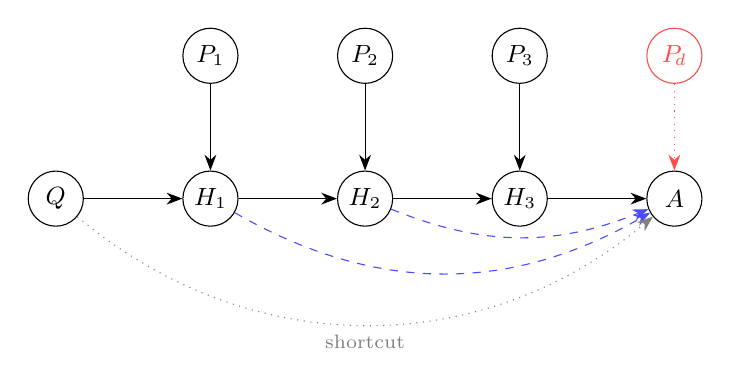
\begin{tikzpicture}[node distance=1.1cm and 1.25cm, every node/.style={font=\small},
  v/.style={draw,circle,minimum size=7mm,inner sep=0pt}, ar/.style={-{Stealth[length=2mm]}}]
\node[v] (q) {$Q$};
\node[v,right=of q] (h1) {$H_1$};
\node[v,right=of h1] (h2) {$H_2$};
\node[v,right=of h2] (h3) {$H_3$};
\node[v,right=of h3] (a) {$A$};
\node[v,above=of h1] (p1) {$P_1$};
\node[v,above=of h2] (p2) {$P_2$};
\node[v,above=of h3] (p3) {$P_3$};
\node[v,above=of a,draw=red!70,text=red!70] (pd) {$P_{\!d}$};
\draw[ar] (q)--(h1); \draw[ar] (h1)--(h2); \draw[ar] (h2)--(h3); \draw[ar] (h3)--(a);
\draw[ar] (p1)--(h1); \draw[ar] (p2)--(h2); \draw[ar] (p3)--(h3);
\draw[ar,dashed,blue!70] (h1) to[bend right=30] (a);
\draw[ar,dashed,blue!70] (h2) to[bend right=22] (a);
\draw[ar,dotted,red!70] (pd)--(a);
\draw[ar,dotted,gray] (q) to[bend right=40] node[below,font=\scriptsize]{shortcut} (a);
\end{tikzpicture}
\caption{Task SCM. Solid: bridge chain. Dashed blue: extra edges of compositional chains. Red
dotted: spurious distractor path that the \emph{reader} may use but the task graph forbids. Gray:
parametric shortcut. CAD's contrast includes the red path; \hgcd{} holds $P$ fixed and contrasts
interventions on $H_j$ only.}
\label{fig:scm}
\end{figure}

\paragraph{Directed reasoning graph (DRG).} Given a generated chain $y=(h_1,\dots,h_k)$ we add an
edge $i\to j$ ($i<j$) if the result of $h_i$ is mentioned in the body of $h_j$. Terminal hops are
those whose result is the query target (CLUTRR) or the last hop (MuSiQue); the \emph{relevant set}
$\Rel(y)$ contains the terminal hops and their DRG ancestors. Hops outside $\Rel(y)$ have no
directed path to the answer.

\paragraph{Interventions on hops.}
\begin{definition}[Naive and graph-aware interventions]
$\donai{j}$ replaces hop $j$ by a mask token and leaves all other hops unchanged.
$\dotot{j}$ masks hop $j$ and, in every DRG descendant $d$ of $j$, masks every mention of the
results of $j$ and of $d$. The latter is a deterministic, rollout-free approximation of
$\mathrm{do}(H_j{=}\bot)$: descendant values are functions of $h_j$, hence unknown under the
intervention. A \emph{placebo} rewrites hop $j$ without changing its entities or relation.
\end{definition}
For an answer $a$ we write $\Delta^{\mathrm{nai}}_j(a)=\pa(a\mid y)-\pa(a\mid\donai{j})$ and
$\Delta^{\mathrm{tot}}_j(a)=\pa(a\mid y)-\pa(a\mid\dotot{j})$, suppressing $Q,P$.

\paragraph{What is (and is not) causal here.} We do not assume the language model \emph{is} an SCM
of the task. The reader $\pa$ is a deterministic function of its input, so editing hops in the
prompt is an exact intervention on the reader's input, and $\Delta_j$ is an exact (not estimated)
effect \emph{on the reader}. The task SCM only supplies ground truth: which hops are necessary,
and which input changes should have no effect on the answer.

\paragraph{Mask-token artifacts.} Replacing text by \texttt{[MASKED]} is itself out of
distribution. Our estimator benchmark controls for this: the inserted redundant hop is masked in
exactly the same way, so any effect caused by the mask token alone appears as a non-zero
$\Delta$ on redundant hops and lowers the AUC. In addition, a \emph{mask-marker} control inserts
\texttt{[MASKED]} into hop $j$ while keeping all of its content; its effect
$\Delta^{\mathrm{marker}}_j$ measures the mask-token artifact directly and should be $\approx0$.

% ===================================================================================
\section{Method: Hop-Graph Contrastive Decoding}
\label{sec:method}

\paragraph{Answer-level rule (L2).} With uniform weights $w_j=1/|\Rel(y)|$ on relevant hops and a
plausibility set $\mathcal{V}_\beta=\{a:\pa(a\mid y)\ge\beta\max_{a'}\pa(a'\mid y)\}$
\citep{li2023contrastive},
\begin{equation}
\begin{aligned}
\hat a&=\arg\max_{a\in\mathcal{V}_\beta}\; s_\alpha(a),\\
s_\alpha(a)&=(1+\alpha)\,\pa(a\mid y)-\alpha\!\!\sum_{j\in\Rel(y)}\!\!w_j\,\pa(a\mid\dotot{j})
=\pa(a\mid y)+\alpha\!\!\sum_{j\in\Rel(y)}\!\!w_j\,\Delta^{\mathrm{tot}}_j(a).
\end{aligned}
\label{eq:hgcd}
\end{equation}
The score is the answer probability plus $\alpha$ times the average total effect of the
answer-relevant hops on that answer. Redundant hops ($j\notin\Rel(y)$) are never contrasted.

\paragraph{Evidence-level rule (L1).} While emitting the \emph{result} tokens of a hop, we contrast
the real context $P$ with a type-matched counterfactual $\tilde P$ of identical length and entity
types in which the relational content differs (on CLUTRR: names permuted within each gender
group, so every sentence and entity type is kept but who-is-related-to-whom changes; we evaluate
L1 on CLUTRR only, where $\tilde P$ is exactly type-matched):
$t^\star=\arg\max_{t\in\mathcal V_\beta}(1{+}\alpha)\pa(t\mid P,\cdot)-\alpha\pa(t\mid\tilde P,\cdot)$.
Unlike an empty context, $\tilde P$ is in-distribution and controls for length and type cues.

\begin{algorithm}[t]
\caption{\hgcd{} (L2) for one question}
\label{alg:hgcd}
\begin{algorithmic}[1]
\State $y\gets$ greedy chain from the model (optionally with L1 contrast on result tokens)
\State Parse hops; build DRG; compute relevant set $\Rel(y)$
\State $p\gets\pa(\cdot\mid Q,P,y)$ over $\mathcal{A}$ \Comment{one forward + KV-cached candidates}
\For{$j\in\Rel(y)$} \State $p_j\gets\pa(\cdot\mid Q,P,\dotot{j})$ \EndFor
\State \Return $\arg\max_{a\in\mathcal{V}_\beta}(1+\alpha)p(a)-\alpha\,\mathrm{mean}_j\,p_j(a)$
\end{algorithmic}
\end{algorithm}

\begin{remark}[What each level can fix]\label{rem:scope}
L2 makes the answer depend \emph{more} on the chain; it therefore repairs \emph{readout} errors
(chain correct, answer wrong because a shortcut or distractor dominates the readout) but cannot
repair a wrong chain---it may even commit harder to one. Chain errors are the target of L1, which
acts while the hops are produced. We test this split directly (\cref{h:readout}).
\end{remark}

\paragraph{Cost.} L2 needs $1+|\Rel(y)|$ prefix forwards and a KV-cached pass over the candidate
tokens; no extra generation. L1 doubles the forward cost of result tokens only.
\paragraph{Choice of $\alpha$.} $\alpha$ is selected on the CLUTRR validation split and frozen
(ties broken toward the smaller $\alpha$, so \hgcd{} reduces to CoT absent evidence); an
adaptive variant sets $\alpha\cdot\mathrm{JSD}(p,\bar p_j)$ as in AdaCAD~\citep{wang2025adacad}.

% ===================================================================================
\section{Theory}
\label{sec:theory}

All proofs are short and given in \cref{app:proofs}; the propositions make predictions that our
protocol tests directly.

\begin{assumption}[Markov reader on bridge chains]\label{as:markov}
For bridge chains, $\pa(a\mid h_{1:k})$ depends on $h_{1:j}$ only through $h_{j+1:k}$ whenever
$h_{j+1}$ restates the result of $h_j$ ($j<k$).
\end{assumption}

\begin{proposition}[Naive masking is a direct effect]\label{prop:direct}
$\Delta^{\mathrm{nai}}_j(a)$ equals the controlled direct effect of $H_j$ on $A$ with
$H_{j+1:k}$ held at their observed values. Under \cref{as:markov}, $\Delta^{\mathrm{nai}}_j(a)=0$
for every $j<k$ on bridge chains, whereas $\Delta^{\mathrm{tot}}_j(a)$ is not constrained to zero.
On compositional chains, where $A$ reads each hop's relation, the direct effect is generally
non-zero.
\end{proposition}
\emph{Prediction.} On CLUTRR both estimators separate necessary from redundant hops; on MuSiQue,
$\Delta^{\mathrm{nai}}\approx0$ on non-final gold hops while $\Delta^{\mathrm{tot}}$ remains large,
so the gap between the two appears in the position breakdown of \cref{tab:est}.

\begin{assumption}[Mixture reader]\label{as:mixture}
$\pa(a\mid Q,P,y)=\lambda_c\pa_c(a\mid y,P_{\mathrm{sup}})+\lambda_s\pa_s(a\mid Q)+
\lambda_d\pa_d(a\mid P_{\mathrm{dist}})$, with $\lambda$'s non-negative, summing to one, and
invariant to interventions on hops.
\end{assumption}

\begin{proposition}[Exact cancellation in probability space]\label{prop:mixture}
Under \cref{as:mixture},
\[
s_\alpha(a)=\pa(a\mid y)+\alpha\lambda_c\sum_j w_j\big[\pa_c(a\mid y)-\pa_c(a\mid\dotot{j})\big],
\]
i.e.\ the shortcut $\pa_s$ and distractor $\pa_d$ components cancel in the contrast for every
$\alpha$. The log-space analogue does not cancel them.
\end{proposition}

\begin{proposition}[CAD amplifies distractor paths]\label{prop:cad}
Under \cref{as:mixture} applied to direct answering, with no-context distribution $\pa_s(a\mid Q)$,
CAD's score is $(1{+}\alpha)\log\big[\lambda_c\pa_c+\lambda_s\pa_s+\lambda_d\pa_d\big](a)-
\alpha\log\pa_s(a\mid Q)$. For any $\alpha>0$ and any gold answer $g$, a distractor answer $a_d$ with
$\pa_d(a_d)=1$ is preferred by CAD whenever $\pa_s(a_d\mid Q)$ is small enough, even if
$\pa(g\mid Q,P)>\pa(a_d\mid Q,P)$. In contrast, \hgcd{}'s contrast term does not depend on
$\pa_d$ at all (\cref{prop:mixture}).
\end{proposition}
\emph{Prediction.} Under distractor injection, CAD's accuracy degrades more than \hgcd{}'s, i.e.\
$|\mathrm{ATE}_{\mathrm{distract}}|$ is larger for CAD.

\begin{proposition}[PNS limit]\label{prop:pns}
Interpret $\pa(a\mid\dotot{j})$ as $P(A{=}a\mid\mathrm{do}(H_j{=}\bot))$ and assume exogeneity and
monotonicity as in \citet{yu2025pns}. Then $\Delta^{\mathrm{tot}}_j(a)=\mathrm{PNS}_j(a)$ and
$\lim_{\alpha\to\infty}s_\alpha(a)/\alpha=\sum_{j\in\Rel(y)}w_j\,\mathrm{PNS}_j(a)$. Hence, within
$\mathcal{V}_\beta$, \hgcd{} interpolates between the most probable answer ($\alpha{=}0$) and the
answer for which the relevant hops are, on average, most necessary and sufficient.
\end{proposition}

% ===================================================================================
\section{Experimental Protocol}
\label{sec:protocol}

\paragraph{Data.} \textbf{CLUTRR}~\citep{sinha2019clutrr} (\texttt{gen\_train234\_test2to10}),
restricted to clean simple-path stories (the filter is reported), gives exact gold paths; ID
$k\in\{2,3,4\}$, OOD $k\ge 5$; answers are scored over the 20 kinship relations.
\textbf{MuSiQue-Ans}~\citep{trivedi2022musique} gives real text with gold decompositions; the
context holds the supporting paragraphs plus 4 distractors. MuSiQue was built to resist
single-hop shortcuts~\citep{min2019compositional}, which is why we prefer it to HotpotQA.
Candidates for MuSiQue are built without the gold answer: the model's own answer and hop results,
then paragraph titles, capitalised spans and dates/numbers from the context, in order of
appearance, capped at 64 (recall of the gold answer is 56\% on 600 dev questions before adding
the model's strings, versus 10.5\% for titles alone). All methods share the same candidate set
and we report its recall.

\paragraph{Binary interventions with known effects.}
\begin{center}\small
\begin{tabular}{lll}
\toprule
Intervention & Definition (programmatic, seeded) & True effect on $A$ \\
\midrule
\texttt{rename} & all names $\to$ fresh fictional names (gender-preserving) & 0 \\
\texttt{order} & shuffle story sentences / paragraphs & 0 \\
\texttt{distract} / \texttt{dist8} & insert a disconnected family / 4 extra distractor paragraphs & 0 \\
\texttt{placebo\_input} & insert two neutral sentences without entities & 0 \\
redundant hop & insert a true but off-path fact as a hop of a gold chain & necessity 0 \\
\bottomrule
\end{tabular}
\end{center}
For each method we report the paired ATE $\mathbb{E}[Y(1)-Y(0)]$ on accuracy with bootstrap 95\%
CIs; a robust method has ATE $\approx0$. \texttt{placebo\_input} controls for ``any change hurts''.

\paragraph{Estimator validation.} Gold chains with one inserted redundant hop give hop-level labels
(necessary $=1$, redundant $=0$). We report AUC of $\Delta^{\mathrm{tot}}$, $\Delta^{\mathrm{nai}}$,
the placebo and mask-marker $\Delta$, rollout PNS~\citep{yu2025pns} and the DRG path indicator, overall and on
chains the model answers correctly ($\mathrm{PS}=1$), and mean effects by hop position.

\paragraph{Methods.} Direct answering; CoT; self-consistency~\citep{wang2023selfconsistency}
with 5 sampled chains (strictly more compute than \hgcd{}, which generates nothing extra);
CAD~\citep{shi2024cad}; AdaCAD~\citep{wang2025adacad};
CAD-chain (contrast with vs.\ without the chain, a text analogue of rationale-conditioned
decoding); \hgcd{} and ablations: naive masking, no graph (all hops), log space, adaptive $\alpha$,
placebo contrast (the key control); L1 chains decoded with CoT or \hgcd{}.

\paragraph{Hypotheses.} The following hypotheses and decision criteria were fixed in the
repository before any GPU experiment was run (verifiable in the commit history).
\begin{hypothesis}[Estimator]\label{h:est} AUC$(\Delta^{\mathrm{tot}})\ge0.75$ on both datasets;
$\Delta^{\mathrm{nai}}$ near zero on MuSiQue non-final gold hops; placebo and mask-marker
$\Delta\approx0$ on all hops.
\end{hypothesis}
\begin{hypothesis}[Accuracy] \hgcd{} $>$ CoT and $>$ CAD-chain on OOD CLUTRR ($k\ge5$) and on
MuSiQue, with paired bootstrap CIs excluding zero.\end{hypothesis}
\begin{hypothesis}[Robustness] $|\mathrm{ATE}_{\mathrm{distract}}|$ of \hgcd{} $<$ that of CAD
(\cref{prop:cad}); ATE of \texttt{placebo\_input} $\approx 0$ for all methods.\end{hypothesis}
\begin{hypothesis}[Readout]\label{h:readout} The gain of \hgcd{} over CoT is concentrated on
questions whose greedy chain reaches every gold-path entity, and is $\approx0$ (or negative) on
the others (\cref{rem:scope}).\end{hypothesis}
\begin{hypothesis}[Ablations] \hgcd{} $\ge$ naive-mask and no-graph variants; probability space
$\ge$ log space; and, crucially, \hgcd{} $>$ placebo contrast. Contrasting against \emph{any}
perturbation can move decisions (our CPU pilot shows this), so the placebo contrast, not CoT, is
the control that isolates the causal content of the intervention.\end{hypothesis}

\paragraph{Models and compute.} Qwen2.5-1.5B-Instruct~\citep{qwen2025qwen25} (main) and
SmolLM2-1.7B-Instruct~\citep{allal2025smollm2} (second family) on two Kaggle T4 GPUs in fp16;
Qwen2.5-7B-Instruct on one A100 for the scale point. Greedy decoding; $\beta=0.1$;
$\alpha\in\{0,0.25,0.5,1,2,4\}$ chosen per method on the CLUTRR validation split and transferred
unchanged to MuSiQue (no MuSiQue data is used for tuning).

\paragraph{Statistics.} Bootstrap CIs (2{,}000 resamples), paired bootstrap differences and exact
McNemar tests on the same questions. The three \emph{primary} comparisons are \hgcd{} vs.\ CoT,
vs.\ CAD-chain and vs.\ the placebo contrast, on OOD CLUTRR and on MuSiQue; all other contrasts
are exploratory and are reported without multiplicity claims. With $n$ questions per split, the half-width of a 95\% CI on
accuracy is about $1/\sqrt{n}$; paired tests are considerably tighter.

% ===================================================================================
\section{Results}
\label{sec:results}

\emph{All tables are produced by the released notebook and \texttt{tools/summarize\_runs.py};
nothing is typed by hand.} Setup: two models (Qwen2.5-1.5B-Instruct, SmolLM2-1.7B-Instruct), fp16,
one Kaggle T4 each; 238 CLUTRR test questions (118 ID, 120 OOD), 120 MuSiQue questions;
estimator benchmark on 90 CLUTRR and 80 MuSiQue gold chains (one inserted redundant hop each).

\begin{table}[h]
\centering\small
\caption{Main quantities, replicated across two model families (effects and accuracies in
points; AUC for separating necessary from redundant hops).}
\label{tab:replication}
\maybeinput{\repdir/tab_replication.tex}
\end{table}

\paragraph{F1: chains are read, not reasoned over (H11 supported).} The chain's content effect on
$p(\text{gold})$ (real chain minus a chain of the same shape with every hop masked) is
$56$--$72$ points on MuSiQue, where the answer is the result written in the last hop, but only
$0.8$--$2.0$ points on CLUTRR, where the answer is a relation that must be composed from the
hops and never appears in them (\cref{tab:replication}). The binary intervention
$T_{\text{copy}}$, which appends one hop stating the answer and leaves everything else identical,
raises the CLUTRR content effect to $75.1$ (Qwen) and $62.8$ (SmolLM2) points. Two further facts
point the same way: on the model's own chains, reaching every gold-path entity does not raise
CLUTRR accuracy (Qwen: $17.1\%$ with gold-path chains vs.\ $18.3\%$ otherwise; SmolLM2:
$15.2\%$ vs.\ $22.4\%$; \cref{tab:readout}), and the chain's \emph{form} has no effect
($0.2$ and $-2.1$ points; \cref{tab:formcontent}). At this scale a chain functions as a place to
look up an answer, not as a computation the model carries out.

\paragraph{F2: direct-effect estimators miss bridge steps (H1, H-validity supported).} Whenever
the answer is copied (MuSiQue, CLUTRR with $T_{\text{copy}}$), masking one non-final hop changes
$p(\text{gold})$ by $-3.6$ to $1.3$ points, while masking it with its DRG descendants changes it
by $66$--$76$ points, close to the effect of the final hop. Two independent total-effect
implementations (masking, counterfactual replacement with propagation) agree (AUC $0.975$--$1.000$),
and both direct variants fail ($0.64$--$0.83$). Placebo rewrites and the mask-marker control stay
at chance on every dataset and model (\cref{tab:est}), so the effects are not artifacts of the
mask token or of rewording.

\paragraph{F3: reasoning relocates vulnerability (H6 supported; \cref{prop:cad} not supported).}
On MuSiQue, distractors lower CoT's exact match by $9.2$ (Qwen) and $7.5$ (SmolLM2) points. Holding
the original chain fixed removes the entire effect (NDE $+0.8$ and $+1.7$); it flows through the
regenerated chain (NIE $-10.0$ and $-9.2$; \cref{tab:mediation}). Every chain-based reader,
including \hgcd{}, CAD-chain, calibration and the direct$\times$CoT product, shows the same
pattern. Direct answering has no chain to corrupt but is hurt at the readout (NDE $-4.2$ and
$-6.7$). With the chain fixed, CAD's readout is no more fragile than direct answering, so the
mechanism of \cref{prop:cad} does not appear at this scale.

\paragraph{F4: decoding cannot amplify dependence that does not exist (H2 not supported; H8
supported).} \hgcd{} matches CoT on both datasets and models ($|\Delta|\le1.7$ points, all
$p\ge0.6$). The only decoding rule that beats CoT on CLUTRR is content-free label calibration
(Qwen $+5.9$ points, McNemar $p=0.009$ against \hgcd{}; SmolLM2 $+3.4$, n.s.), which uses no
information about the chain at all and is itself fragile (ATE of the neutral-sentence placebo
$-5.0$ [$-10.1$, $-0.4$] for SmolLM2). The earlier gains of the naive-mask and log-space
variants at $\alpha=4$ are of this kind. CLUTRR errors at this scale are dominated by the label
prior, which F1 explains: the model is not using the chain to compute the relation.

\begin{table}[h]
\centering\small
\caption{Hypothesis scorecard after two GPU rounds.}
\label{tab:scorecard}
\begin{tabular}{p{0.33\linewidth}p{0.45\linewidth}c}
\toprule
Hypothesis & Evidence (both models) & Verdict \\
\midrule
H1 estimator validity (copyable answers) & AUC $0.975$--$1.000$ total vs.\ $0.64$--$0.83$ direct & \checkmark \\
H11 copy, not compute & content $1$--$2\to63$--$75$ points with $T_{\text{copy}}$ & \checkmark \\
H6 mediation & dist8: NIE $-9$ to $-10$, NDE $\approx+1$ for every chain-based reader & \checkmark \\
H8 calibration explains decoding gains & calibration $\ge$ naive/log variants & \checkmark \\
H2 \hgcd{} improves accuracy & $=$ CoT everywhere & $\times$ \\
H3 / \cref{prop:cad} CAD more fragile at readout & CAD NDE $\approx$ direct NDE & $\times$ \\
H-form chain form explains CoT gains & form effect $0.2$ / $-2.1$ points & $\times$ \\
H4 readout & gold-path chains do not raise accuracy (supports F1, not \hgcd{}) & -- \\
H-scale, H-niche & require the scale study (\texttt{MODE="reliance"}) & pending \\
\bottomrule
\end{tabular}
\end{table}

\begin{table}[h]
\centering\small
\caption{Estimator validation, Qwen2.5-1.5B (SmolLM2 in \cref{app:smol}).}
\label{tab:est}
\maybeinput{\resultsdir/tab_estimators_auc.tex}\\[4pt]
\maybeinput{\resultsdir/tab_estimators_pos.tex}
\end{table}

\begin{table}[h]
\centering\small
\caption{Form vs.\ content effect of a chain on $p(\text{gold})$, Qwen2.5-1.5B.}
\label{tab:formcontent}
\maybeinput{\resultsdir/tab_form_content.tex}
\end{table}

\begin{table}[h]
\centering\small
\caption{Mediation of distractor and order effects on MuSiQue, Qwen2.5-1.5B (EM points).}
\label{tab:mediation}
\maybeinput{\resultsdir/tab_musique_mediation.tex}
\end{table}

\begin{table}[h]
\centering\small
\caption{CLUTRR accuracy (\%), Qwen2.5-1.5B. ID: $k\le4$; OOD: $k\ge5$.}
\label{tab:clutrr}
\maybeinput{\resultsdir/tab_clutrr_main.tex}
\end{table}

\begin{table}[h]
\centering\small
\caption{CLUTRR accuracy split by whether the model's chain reaches every gold-path entity.}
\label{tab:readout}
\maybeinput{\resultsdir/tab_clutrr_readout.tex}
\end{table}

\begin{table}[h]
\centering\small
\caption{MuSiQue exact match (\%), Qwen2.5-1.5B.}
\label{tab:musique}
\maybeinput{\resultsdir/tab_musique_main.tex}
\end{table}

\subsection{Round-3 hypotheses (fixed before the next run)}
\label{sec:round3}
\begin{hypothesis}[Does computation emerge with scale?]\label{h:scale} The CLUTRR content effect
(without $T_{\text{copy}}$) stays below $10$ points up to 3B and rises above it at 7B; the gap
between total and direct estimators on bridge chains persists at every scale.\end{hypothesis}
\begin{hypothesis}[Copying on the model's own chains]\label{h:copydiag} When the gold relation word
appears in the model's own CLUTRR chain, CoT accuracy is higher and the chosen relation is a word
from the chain more often than when it does not.\end{hypothesis}
\begin{hypothesis}[Copying overrides the chain's own logic]\label{h:wrongcopy} If the appended
hop states a \emph{wrong} relation that contradicts the relational hops before it, the model
follows it in most chains (argmax equals the wrong relation in $>50\%$), i.e.\ it reads the stated
answer instead of checking it against the hops it reads past. A model that computes over the chain
would resist.\end{hypothesis}
\begin{hypothesis}[Cheap total effect]\label{h:cheap} Rollout PNS and graph-aware masking rank hops
consistently (AUC difference $\le0.05$), at about $1/K$ of the cost.\end{hypothesis}

\section{Limitations}
\textbf{Assumptions.} \cref{as:markov,as:mixture} idealise the reader; we treat the propositions as
testable predictions rather than guarantees, and the protocol is designed to falsify them.
\textbf{Rollout-free interventions.} $\dotot{j}$ approximates $\mathrm{do}(H_j)$ by masking rather
than re-generating descendants; we validate it against rollout PNS where compute allows.
\textbf{Format dependence.} The DRG requires hop-structured chains linked by explicit mentions;
pronouns break links and shrink $\Rel(y)$ to the terminal hop. We report format success, hop
fidelity against the gold path and the fraction of fully connected DRGs, and fall back to CoT
when parsing fails. \textbf{Closed-set scoring.} All CLUTRR methods, including CoT, are scored
over the same 20 relations, so differences are not due to answer extraction. \textbf{Candidate sets.} Answer-level contrast needs a finite
candidate set; it is exact on CLUTRR and approximate on MuSiQue (we report candidate recall).
\textbf{Scale.} Main experiments use 1.5--7B models; larger models may rely less on shortcuts.
\textbf{Data filter.} We use CLUTRR stories whose gold graph is a simple path; stories with
back-edges contain known label ambiguities.

\section{Conclusion}
With interventions whose ground truth is known, we find that 1.5--1.7B models use their reasoning
chains as a place to read an answer, not as a computation: the dependence appears exactly when the
answer is written in the chain and can be switched on by writing it there. Measuring this
correctly requires graph-aware total-effect interventions, because single-step masking misses
bridge reasoning entirely. Chain-of-thought moves a model's vulnerability to distractors from the
readout to chain generation, which is why decoding rules that act on the readout, including the
one we propose, do not help at this scale. Whether computation over the chain emerges with scale is
the question our released protocol is designed to answer next.

\bibliographystyle{plainnat}
\bibliography{refs}

\appendix
\section{Proofs}
\label{app:proofs}

\paragraph{\Cref{prop:direct}.} $\donai{j}$ changes only $h_j$ and keeps $h_{j+1:k}$ at their
observed values, so $\Delta^{\mathrm{nai}}_j$ is by definition the controlled direct effect
$\pa(a\mid h_j,h_{-j})-\pa(a\mid\bot,h_{-j})$~\citep{pearl2001direct}. Under \cref{as:markov},
$\pa(a\mid h_{1:k})=g(a\mid h_{j+1:k})$ for $j<k$, so both terms equal $g(a\mid h_{j+1:k})$ and the
difference is zero. $\dotot{j}$ additionally changes $h_{j+1:k}$ (their results are masked), so
$g$ is evaluated at a different argument and the difference is unconstrained. On compositional
chains $\pa$ reads the relation of every hop, so removing $h_j$ alone changes the composed relation.
$\square$

\paragraph{\Cref{prop:mixture}.} Substituting \cref{as:mixture} into \cref{eq:hgcd}, with
$\sum_j w_j=1$ and $\pa_s,\pa_d$ unaffected by interventions on hops:
$s_\alpha(a)=(1{+}\alpha)[\lambda_c\pa_c(a\mid y)+\lambda_s\pa_s+\lambda_d\pa_d]-
\alpha\sum_j w_j[\lambda_c\pa_c(a\mid\dotot{j})+\lambda_s\pa_s+\lambda_d\pa_d]
=\pa(a\mid y)+\alpha\lambda_c\sum_jw_j[\pa_c(a\mid y)-\pa_c(a\mid\dotot{j})]$.
In log space, $\log(\lambda_c u+r)-\log(\lambda_c v+r)$ depends on $r=\lambda_s\pa_s+\lambda_d\pa_d$
unless $u=v$, so the shortcut terms do not cancel. $\square$

\paragraph{\Cref{prop:cad}.} Let $m(a)=\pa(a\mid Q,P)$. CAD prefers $a_d$ over $g$ iff
$(1{+}\alpha)\log\frac{m(a_d)}{m(g)}>\alpha\log\frac{\pa_s(a_d)}{\pa_s(g)}$. The left side is
bounded below by $(1{+}\alpha)\log\frac{\lambda_d}{m(g)}$ since $m(a_d)\ge\lambda_d$, while the right
side tends to $-\infty$ as $\pa_s(a_d)\to0$. For \hgcd{}, both terms of \cref{eq:hgcd} condition
on the same $P$, so $\lambda_d\pa_d$ enters both and cancels (\cref{prop:mixture}). $\square$

\paragraph{\Cref{prop:pns}.} Under exogeneity and monotonicity, Lemma 2 of \citet{yu2025pns}
gives $\mathrm{PNS}=P(A{=}a\mid\mathrm{do}(S))-P(A{=}a\mid\mathrm{do}(S'))$. With $S=y$ and $S'=\dotot{j}$
this is $\Delta^{\mathrm{tot}}_j(a)$. Dividing \cref{eq:hgcd} by $\alpha$ and letting
$\alpha\to\infty$ removes the $\pa(a\mid y)/\alpha$ term. $\square$

\section{Implementation and Reproducibility}
\label{app:impl}
Candidate log-probabilities are computed with one prefix forward and a KV-cached pass over the
candidate tokens (verified against full recomputation to $2\times10^{-5}$). Prompts are two-shot,
hop-structured; the second CLUTRR shot uses a relation outside the label set to avoid leaking label
statistics. All interventions are seeded functions of the example id. The Kaggle notebook embeds
the full package and writes every table in this paper.

\section{SmolLM2-1.7B tables}
\label{app:smol}
\begin{center}\small
\maybeinput{\smoldir/tab_estimators_auc.tex}\\[6pt]
\maybeinput{\smoldir/tab_estimators_pos.tex}\\[6pt]
\maybeinput{\smoldir/tab_form_content.tex}\\[6pt]
\maybeinput{\smoldir/tab_musique_mediation.tex}\\[6pt]
\maybeinput{\smoldir/tab_clutrr_main.tex}
\end{center}

\section{Pilot run (pipeline sanity check)}
\label{app:pilot}
The following tables come from a CPU smoke run with Qwen2.5-0.5B-Instruct on a handful of
examples. They verify that the pipeline runs end to end and are \textbf{not} evidence for or against
any hypothesis.

\begin{center}\small
\maybeinput{\pilotdir/tab_estimators_auc.tex}\\[6pt]
\maybeinput{\pilotdir/tab_estimators_pos.tex}\\[6pt]
\maybeinput{\pilotdir/tab_clutrr_main.tex}
\end{center}
Even at this scale, the position breakdown shows the qualitative pattern predicted by
\cref{prop:direct} on MuSiQue: naive masking leaves the answer probability of non-final gold
hops nearly unchanged, whereas graph-aware masking reduces it substantially. With a few dozen
hops this is an illustration, not a test.

\end{document}
